\documentclass[sigplan,anonymous,review,protrusion=true,expansion]{acmart}

\usepackage[utf8]{inputenc}
\usepackage[T1]{fontenc}
\usepackage{mathtools}
\usepackage{enumerate}

% Céu.
\newcommand{\CEU}{\textsc{C\'{e}u}\xspace}

% Notes
\usepackage[textsize=footnotesize]{todonotes}
\newcommand{\rc}[1]{\todo[inline,color=green!40]{\textbf{Rodrigo}: #1}}
\newcommand{\fs}[1]{\todo[inline,color=blue!40]{\textbf{Francisco}: #1}}
\newcommand{\gl}[1]{\todo[inline,color=red!40]{\textbf{Guilherme}: #1}}

% Concrete syntax.
\usepackage{listings}
\lstdefinelanguage{ceu}{%
  language=C,
  morekeywords={%
    @const, @pure, @safe, CHAN, FOREVER, PAR, PROC, SIGNAL, abort, and,
    await, bool, call, class, data, define, deterministic, do, each, else,
    emit, end, escape, event, every, finalize, hor, implementation, in,
    input, interface, loop, min, native, new, nohold, not, or, output, par,
    pool, pure, return, s, signal, spawn, tag, then, this, traverse, until,
    var, watching, when, with},
}
\lstset{
  basicstyle=\ttfamily,
  captionpos=b,
  columns=flexible,
  commentstyle=\rmfamily\itshape,
  escapeinside={||},
  frame=tb,
  keepspaces=true,
  keywordstyle=\bfseries,
  language=ceu,
  mathescape=true,
  numbersep=4pt,
  numberstyle=\scriptsize,
  upquote=true,
}
\newcommand{\code}[1]{{\small{\texttt{#1}}}}
%\let\code\lstinline
\usepackage{xspace}
\newcommand{\ax}{\code{[a]}\xspace}
\newcommand{\bx}{\code{[b]}\xspace}

% Abstract syntax.
\makeatletter
\def\@int{\mathit{int}}
\def\@ext{\mathit{ext}}
\def\@ceuop#1{\mathop{\normalfont{\texttt{#1}}}}%
\def\@ceubin#1{\mathbin{\normalfont{\texttt{#1}}}}%
\def\ceu{\protect\@ceu}
\def\@ceu#1{%
  \bgroup
  \def\Id{\mathit{id}}%
  \def\Mem{\@ceuop{mem}}%
  \def\AwaitExt{\@ceuop{await}\nolimits_\@ext}%
  \def\AwaitInt{\@ceuop{await}\nolimits_\@int}%
  \def\EmitInt{\@ceuop{emit}\nolimits_\@int}%
  \def\Break{\@ceuop{break}}%
  \def\Ifelse##1##2##3{\@ceuop{if}##1\@ceuop{then}{##2}\@ceuop{else}{##3}}%
  \def\Loop{\@ceuop{loop}}%
  \def\Every{\@ceuop{every}}%
  \def\And{\@ceubin{and}}%
  \def\Or{\@ceubin{or}}%
  \def\Fin{\@ceuop{fin}}%
  \def\AtLoop{\@ceuop{@loop}}%
  \def\AtAnd{\@ceubin{@and}}%
  \def\AtOr{\@ceubin{@or}}%
  \def\CanRun{\@ceuop{@canrun}}%
  \def\Nop{\@ceuop{@nop}}%
  \ensuremath{#1}\ignorespaces
  \egroup
}
\makeatother

% Copyright
%\setcopyright{none}
%\setcopyright{acmcopyright}
%\setcopyright{acmlicensed}
\setcopyright{rightsretained}
%\setcopyright{usgov}
%\setcopyright{usgovmixed}
%\setcopyright{cagov}
%\setcopyright{cagovmixed}

% DOI
\acmDOI{10.475/123_4}

% ISBN
\acmISBN{123-4567-24-567/08/06}

%Conference
\acmConference[WOODSTOCK'97]{ACM Woodstock conference}{July 1997}{El
  Paso, Texas USA}
\acmYear{1997}
\copyrightyear{2016}

\acmPrice{15.00}

%\acmBadgeL[http://ctuning.org/ae/ppopp2016.html]{ae-logo}
%\acmBadgeR[http://ctuning.org/ae/ppopp2016.html]{ae-logo}

\begin{document}

\title[A Memory-Bounded, Deterministic, and Terminating Semantics for \CEU]
{A Deterministic and Terminating Semantics
  for the Synchronous Programming Language~\CEU}

\author[R.\,C.\,M.~Santos]{Rodrigo C.\,M.~Santos}
\email{rsantos@inf.puc-rio.br}
\affiliation{PUC-Rio, Rio de Janeiro, Brazil}
%
\author[G.\,F.~Lima]{Guilherme F.~Lima}
\email{glima@inf.puc-rio.br}
\affiliation{PUC-Rio, Rio de Janeiro, Brazil}
%
\author[F.~Sant'Anna]{Francisco Sant'Anna}
\email{francisco@ime.uerj.br}
\affiliation{UERJ, Rio de Janeiro, Brazil}
%
\author[R.~Ierusalimschy]{Roberto Ierusalimschy}
\email{roberto@inf.puc-rio.br}
\affiliation{PUC-Rio, Rio de Janeiro, Brazil}
%
\author[E.\,H.~Haeusler]{Edward Hermann Haeusler}
\email{hermann@inf.puc-rio.br}
\affiliation{PUC-Rio, Rio de Janeiro, Brazil}

\begin{abstract}
\CEU is a synchronous programming language for embedded soft real-time systems.
%
It focus on control-flow safety features, such as safe shared-memory
concurrency and safe abortion of lines of execution, while enforcing
memory-bounded, deterministic, and terminating reactions to the environment.
%
In this work, we present a small-step structural operational semantics for
\CEU and a proof that reactions have the properties enumerated above:
%
that for a given arbitrary timeline of input events, multiple executions of the
same program always react in bounded time and arrive at the same final finite
memory state.
%
%We also discuss some equivalence results and the relation between the proposed
%semantics and its actual implementation.
\end{abstract}

\terms{Languages, design, theory}
\keywords{Operational semantics, \CEU, Synchronous languages}

\begin{CCSXML}
<ccs2012>
 <concept>
  <concept_id>10003752.10010124.10010131.10010134</concept_id>
  <concept_desc>Theory of computation~Operational semantics</concept_desc>
  <concept_significance>500</concept_significance>
 </concept>
 <concept>
  <concept_id>10011007.10011006.10011008.10011009.10011014</concept_id>
  <concept_desc>Software and its
                engineering~Concurrent programming languages</concept_desc>
  <concept_significance>500</concept_significance>
 </concept>
 <concept>
  <concept_id>10010520.10010553.10010562.10010564</concept_id>
  <concept_desc>Computer systems
                organization~Embedded software</concept_desc>
  <concept_significance>300</concept_significance>
 </concept>
</ccs2012>
\end{CCSXML}
\ccsdesc[500]{Theory of computation~Operational semantics}
\ccsdesc[500]{Software and its engineering~Concurrent programming languages}
\ccsdesc[300]{Computer systems organization~Embedded software}

\maketitle

\section{Introduction}
\label{sec.intro}

\CEU~\cite{ceu.sensys13,ceu.tecs17} is a Esterel-based~\cite{esterel.ieee91}
programming language for embedded soft real-time systems that aims to offer a
concurrent, safe, and expressive alternative to C with the characteristics that
follow:
%
\begin{description}
\item [Reactive:] code only executes in reactions to events.
\item [Structured:] programs use structured control mechanisms, such as
    \code{await} (to suspend a line of execution), and \code{par} (to combine
    multiple lines of execution).
\item [Synchronous:] reactions run atomically and to completion on each line of
    execution, i.e., there's no implicit preemption or real parallelism.
\end{description}
%
Structured reactive programming let developers write code in direct/sequential
style, recovering from the inversion of control imposed by event-driven
execution~\cite{rp.deprecating,rp.rescala,sync_async.cooperative}.
%
Synchronous languages offer a simple run-to-completion model of execution that
enable deterministic execution and make formal reasoning tractable.
For this reason, it has been successfully adopted in safety-critical real-time
embedded systems.~\cite{rp.twelve}

Previous work in the context of embedded sensor networks evaluates the
expressiveness of \CEU in comparison to event-driven code in C and attests a
reduction in source code size (around 25\%) with a small increase in memory
usage (around 5--10\% for \emph{text} and \emph{data})~\cite{ceu.sensys13}.
%
\CEU has also been used in the context of multimedia
systems~\cite{ceumedia.webmedia16} and games~\cite{ceu.mod15}, and as an
alternative language in an undergraduate-level course on embedded systems for
the past 6 years.

\CEU inherits the synchronous and imperative mindset of Esterel but adopts a
simpler semantics with fine-grained execution control.~\cite{ceu.tecs17}
%
The list that follows summarizes the semantic peculiarities of \CEU:
%
\begin{itemize}
    \item Stack-based execution for internal events, which provides a limited
          form of coroutines.
    \item Fine-grained, intra-reaction deterministic execution, which allows
          programs to safely share memory.
    \item Finalization mechanism for abortion of lines of execution, which
          safely release external resources.
    \item First-class synchronized timers.
\end{itemize}

In this work, we present a formal semantics for a subset of \CEU that focus on
its peculiarities in comparison to other synchronous languages.
\begin{itemize}
    \item qual a abordagem / operational semantics / dois passos
    \item quais os resultados / provas
    \item quais os desafios e limitações
    \item \gl{TODO}
\end{itemize}

\fs{Descrever seções.}

\section{\CEU}
\label{sec.ceu}

\CEU is a synchronous reactive language in which programs advance in a sequence
of discrete reactions to external events.
%
It is designed for control-intensive applications, supporting concurrent lines
of execution, known as \emph{trails}, and instantaneous broadcast communication
through events.
%
Computations within a reaction (such as expressions, assignments, and
system calls) are also instantaneous considering the synchronous
hypothesis~\cite{rp.hypothesis}.
%
%\CEU provides an \code{await} statement which is the only that actually
%``consumes'' time.
%
\CEU provides an \code{await} statement that blocks the current running trail
allowing the program to advance its other trails; when all trails are blocked,
the reaction terminates and control returns to the environment.

In \CEU, every execution path within loops must contain at least one
\code{await} statement to an external input
event~\cite{ceu.sensys13,esterel.primer}.
%
This restriction, which is statically checked by the compiler, ensures that
every reaction runs in bounded time, eventually terminating with all trails
blocked in \code{await} statements.
%
\CEU has an additional restriction, which it shares with Esterel and
synchronous languages in general~\cite{esterel.preemption}: computations that
take a non-negligible time to run (e.g., cryptography or image processing
algorithms) violate the zero-delay hypothesis, and thus cannot be directly
implemented.

Listing~\ref{lst.syntax} shows a compact reference of~\CEU:

\bgroup
\def\T<#1>{\langle\mathit{#1}\rangle}
\def\C#1#2{\hfill\rmfamily\itshape\makebox[#1\columnwidth][l]{//~#2}}
\begin{lstlisting}[
  basicstyle=\ttfamily\footnotesize,
  caption={The concrete syntax of \CEU.},
  label={lst.syntax},
]
|\C{1.}{Declarations}|
input $\T<type>$ $\T<id>$; | \C{.6}{declares an external input event} |
event $\T<type>$ $\T<id>$; | \C{.6}{declares an internal event}       |
var   $\T<type>$ $\T<id>$; | \C{.6}{declares a variable}              |

|\C{1.}{Event handling}|
$\T<id>$ = await $\T<id>$;   | \C{.6}{awaits an event and assigns the received value} |
emit $\T<id>$($\T<exp>$);    | \C{.6}{emits an event passing a value} |

|\C{1.}{Control flow}|
$\T<stmt>$ ; $\T<stmt>$                          | \C{.45}{sequence}     |
if $\T<exp>$ then $\T<stmts>$ else $\T<stmts>$ end    | \C{.45}{conditional}  |
loop do $\T<stmts>$ end                      | \C{.45}{repetition}   |
every $\T<id>$ in $\T<id>$ do $\T<stmts>$ end         | \C{.45}{event iteration}   |
finalize [$\T<stmts>$] with $\T<stmts>$ end       | \C{.45}{finalization} |

|\C{1.}{Logical parallelism}|
par/or  do $\T<stmts>$ with $\T<stmts>$ end | \C{.45}{aborts when any side ends}      |
par/and do $\T<stmts>$ with $\T<stmts>$ end | \C{.45}{terminates when all sides ends} |
par     do $\T<stmts>$ with $\T<stmts>$ end | \C{.45}{never terminates}               |

|\C{1.}{Assignment \& Integration with C}|
$\T<id>$ = $\T<exp>$; | \C{.6}{assigns a value to a variable}              |
_$\T<id>$($\T<exps>$) | \C{.6}{calls a C function (id starts with `\_'\,)} |
\end{lstlisting}
\egroup

Listing~\ref{lst.ceu} shows a complete example in \CEU that toggles a LED
whenever a radio packet is received, terminating with a button press always
with the LED off.
%
The implementation first declares the \code{BUTTON} and \code{RADIO\_RECV} as
input events (ln.~1--2).
Then, it uses a \code{par/or} composition to run two activities in parallel:
a single statement that waits for a button press before terminating (ln.~4),
and an endless loop that toggles the LED on and off on radio receives
(ln.~9--14).
The \code{finalize} clause (ln.~6--8) ensures that, no matter how its enclosing
trail terminates, the LED will be unconditionally turned off (ln.~7).

The \code{par/or} composition, which stands for a \emph{parallel-or}, provides
an orthogonal abortion mechanism~\cite{esterel.preemption} in which its
composed trails do not know when and how they are aborted (i.e., abortion is
external to them).
%
%This is possible to do safely in synchronous languages due to the accurate
%control of concurrent activities, i.e., in between every reaction, the whole
%system is idle and consistent~\cite{esterel.preemption}.
%
The finalization mechanism extends orthogonal abortion to also work with
activities that use stateful resources from the environment (such as files and
network handlers), as we discuss in Section~\ref{sec.ceu.fin}.
%

\begin{lstlisting}[
  numbers=left,
  basicstyle=\ttfamily\footnotesize,
  float=h,
  caption={A program in \CEU that toggles a LED on every radio receive,
           terminating on a button press in a consistent state.},
  label={lst.ceu},
]
input void BUTTON;
input void RADIO_RECV;
par/or do
    await BUTTON;
with
    finalize with
        _led(0);
    end
    loop do
        _led(1);
        await RADIO_RECV;
        _led(0);
        await RADIO_RECV;
    end
end
\end{lstlisting}

In \CEU, any identifier prefixed with an underscore (e.g., \code{\_led}) is
passed unchanged to the underlying~C compiler.
%
Therefore, access to~C is straightforward and syntactically traceable.
%
To ensure that programs operate under the synchronous hypothesis, the compiler
environment should only provide access to~C operations that can be assumed to
be instantaneous, such as non-blocking~I/O and simple accesses to data
structures.

\subsection{External and Internal Events}
\label{sec.ceu.evts}

\CEU defines time as a discrete sequence of reactions to unique external
input events.
%
External input events are received from the environment, and each delimits a
new logical unit of time that triggers an associated reaction.
%
The life-cycle of a program in \CEU can be summarized as
follows~\cite{ceu.sensys13}:
%
\begin{enumerate}[i]
\item The program initiates a ``boot reaction'' in a single trail (parallel
      constructs may create new trails).
\item Active trails execute until they await or terminate, one after
      another.  This step is called a \emph{reaction chain}, and always runs in
      bounded time.
\item When all trails are blocked, the program goes idle and the environment
      takes control.
\item On the occurrence of a new external input event, the environment
      awakes \emph{all} trails awaiting that event, and the program goes back to
      step~(ii).
\end{enumerate}

A program must react to an event completely before handling the next one.
%
By the synchronous hypothesis, the time the program spends in step~(ii) is
conceptually zero (in practice, negligible).
%
Hence, from the point of view of the environment, the program is always
idle on step~(iii).
%
In practice, if a new external input event occurs while a reaction executes,
the event is saved on a queue, which effectively schedules it to be processed
in a subsequent reaction.

\subsubsection*{External events and discrete time}

\begin{figure}[b]
\centering
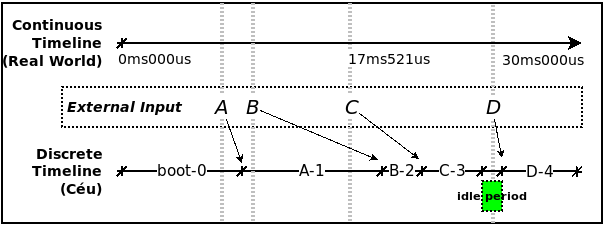
\includegraphics[width=\columnwidth]{tick_min}
\caption{The discrete notion of time in \CEU.}
\label{fig.ticks}
\end{figure}

The sequential processing of external input events induces a discrete notion of
time in \CEU, as illustrated in Figure~\ref{fig.ticks}.
%
The continuous timeline shows an absolute reference clock with ``physical
timestamps'' for the event occurrences (e.g., event~\code{C} occurs at
$17ms521us$).
%
The discrete timeline shows how the same occurring events fit in the logical
notion of time of \CEU.
%
The boot reaction \code{boot-0} happens before any input, at program startup.
%
Event~\code{A} ``physically'' occurs during \code{boot-0} but, because time
is discrete, its corresponding reaction only executes afterwards, at logical
instant~\code{A-1}.
%
Similarly, event~\code{B} occurs during~\code{A-1} and its reaction is
postponed to execute at~\code{B-2}.
%
Event~\code{C} also occurs during~\code{A-1} but its reaction must also wait
for~\code{B-2} to execute and so it is postponed to execute at~\code{C-3}.
%
Finally, event~\code{D} occurs during an idle period and can start immediately
at \code{D-4}.
%
%Finally, two instances of event~\code{E} occur during~\code{D-4}; they are
%handled in the subsequent reactions~\code{E-5} and~\code{E-6}.

Unique input events imply mutually exclusive reactions, which execute
atomically and never overlap.
%
Automatic mutual exclusion is a prerequisite for deterministic reactions as
we discuss in Section~\ref{sec.sem}.
%
%8<- - - - - - - - - - - - - - - - - - - - - - - - - - - - - - - - - - - - -
% \gl{A não ser que seja desenvolvido (e.g., explicado e comparado com
%   Esterel) eu acho que o parágrafo anterior é dispensável.}
% \fs{Tirei o "simplifies resoning about concurrency".
%     O resto do parágrafo é absoluto e tenta dar a intuição das condições para
%     ter determinismo.}
%- - - - - - - - - - - - - - - - - - - - - - - - - - - - - - - - - - - - ->8

In practice, the synchronous hypothesis for \CEU holds if reactions execute
faster than the rate of incoming input events.
%
Otherwise, the program would continuously accumulate delays between physical
occurrences and actual reactions for the input events.
%
Considering the context soft real-time systems,
%targeted by \CEU (e.g., sensor networks, multimedia systems, interactive games, etc.)
such delays and postponed reactions might be tolerated as long as they are
infrequent and the application does not take too long to catch up with real
time.
%
Note that the synchronous semantics is the norm in typical event-driven
systems, such as event dispatching in UI toolkits, game loops in game engines,
and clock ticks in embedded systems.

\subsubsection*{Internal events as subroutines}

In \CEU, queue-based processing of events applies only to external input
events, i.e., events submitted to the program by the environment.
%
Internal events, which are events generated internally by the program via
\code{emit} statements, are processed in a stack-based manner.
%
Internal events provide a fine-grained execution control, and, because of their
stack-based processing, can be used to implement a limited form of subroutines,
as illustrated in Listing~\ref{lst.sub}:

\begin{lstlisting}[
  numbers=left,
  basicstyle=\ttfamily\footnotesize,
  float=h,
  caption={A \CEU program with a ``subroutine''.},
  label={lst.sub},
]
event int* inc;         // declares subroutine "inc"
par/or do
    var int* p;
    every p in inc do   // implements "inc" through an event iterator
        *p = *p + 1;
    end
with
    var int v = 1;
    emit inc(&v);       // calls "inc"
    emit inc(&v);       // calls "inc"
    _assert(v==3);      // asserts result after the two returns
end
\end{lstlisting}
%\vskip-\baselineskip

In the example, the ``subroutine'' \code{inc} is defined as an event iterator
(ln.~4--6) that continuously awaits its identifying event (ln.~4), and
increments the value passed by reference (ln.~5).
%
A trail in parallel (ln.~8--11) invokes the subroutine through two consecutive
\code{emit} statements (ln.~9--10).
%
Given the stack-based execution for internal events, as the first emit
executes, the calling trail pauses (ln.~9), the subroutine awakes (ln.~4), runs
its body (yielding \code{v=2}), iterates, and awaits the next ``call'' (ln.~4,
again).
%
Only after this sequence does the calling trail resumes (ln.~9), makes a new
invocation (ln.~10), and passes the assertion test (ln.~11).

%- multiple executions
%- footnote to distinguish from TECS

\CEU also supports nested \code{emit} invocations, e.g., the body of the
subroutine \code{inc} (ln.~5) could \code{emit} an event targeting another
subroutine, creating a new level in the stack.
%
We can think of the stack as a record of the nested, fine-grained internal
reactions that happen inside the same outer reaction to a single external
event.

This form of subroutines has a significant limitation though: it cannot
express recursion, since an \code{emit} to itself is always ignored as a
running trail cannot be waiting on itself.
%
That being said, it is this very limitation that brings important safety
properties to subroutines.
%
First, they are guaranteed to react in bounded time.
%
Second, memory for locals is also bounded, not requiring data stacks.

At first sight, event iteration such as in ``\code{every e do <...> end}'' seems
to be equivalent to ``\code{loop do await e; <...> end}''.
However, the \code{loop} variation would not compile because it does not
contain a path to an external input \code{await} (\code{e} is an internal
event).
%
However, event iterators enforce syntactic restrictions and cannot contain
\code{await} or \code{break} statements.
The absence of \code{break} guarantees that an iterator never terminates from
itself, essentially behaving as a safe blocking point in the program.
%
For this reason, the restriction that execution paths within loops must
contain at least one external \code{await} is extended to alternatively contain
an \code{every} statement.

\subsection{Shared-Memory Concurrency}

Embedded applications make extensive use of global memory and shared resources,
such as through memory-mapped registers and system calls to device drivers.
Hence, an important goal of \CEU is to ensure a reliable behavior for programs
with concurrent lines of execution sharing memory and interacting with the
environment.

\begin{figure}[h]
\begin{minipage}[h]{0.45\linewidth}
\begin{lstlisting}[numbers=right]
input void A;
input void B;
var int x = 1;
par/and do
    await A;
    x = x + 1;
with
    await B;
    x = x * 2;
end
\end{lstlisting}
\centering\small{\ax Accesses to \code{x} are never concurrent.}
\end{minipage}
%
\begin{minipage}[h]{0.53\linewidth}
%\begin{lstlisting}
\begin{lstlisting}[xleftmargin=2em]
input void A;
// (empty line)
var int y = 1;
par/and do
    await A;
    y = y + 1;
with
    await A;
    y = y * 2;
end

\end{lstlisting}
\centering\small{\bx Accesses to \code{y} are concurrent but deterministic.}
\end{minipage}
%\rule{8.4cm}{0.37pt}
\caption{ Shared-memory concurrency in \CEU:
example \ax is safe because the trails access \code{x} atomically in different
reactions;
example \bx is unsafe because both trails access \code{y} in the same reaction.
\label{lst.shared}
}
\end{figure}

In \CEU, when multiple trails are active during the same reaction, they are
scheduled in lexical order, i.e., in the order they appear in the program
source code.
%
For instance, consider the two examples in Figure~\ref{lst.shared}, both
defining shared variables (ln. 3), and assigning to them in parallel trails
(ln. 6, 9).

In the example \ax, the two assignments to \code{x} can only execute in
reactions to different events \code{A} and \code{B}, which cannot occur
simultaneously by definition (Section~\ref{sec.ceu.evts}).
Hence, for the sequence of events \code{A->B}, \code{x} becomes \code{4}
(\code{(1+1)*2}), while for \code{B->A}, \code{x} becomes \code{3}
(\code{(1*2)+1}).

In the example \bx, the two assignments to \code{y} are simultaneous because
they execute in reaction to the same event \code{A}.
Since \CEU employs lexical order for intra-reaction statements, the execution
is still deterministic, and \code{y} always becomes \code{4} (\code{(1+1)*2}).
%
However, note that an apparently innocuous change in the order of trails
modifies the behavior of the program.
%
To mitigate this threat, \CEU performs concurrency checks at compile time to
detect conflicting accesses to shared variables:
if a variable is written in a trail segment, then a concurrent trail segment
cannot read or write to that variable~\cite{ceu.sensys13}.
%
Nonetheless, the static checks are optional and are not a prerequisite for the
deterministic semantics of the language.

\subsection{Abortion and Finalization}
\label{sec.ceu.fin}

\begin{figure}
\begin{minipage}[t]{0.45\linewidth}
\begin{lstlisting}[numbers=right]
par/or do
   var _msg_t msg;
   <...> // prepare msg
   finalize
      _send(&msg);
   with
      _cancel(&msg);
   end
   await SEND_ACK;
with
   <...>
end
//
\end{lstlisting}
\centering\small{\ax Local resource finalization}
\end{minipage}
%
\begin{minipage}[t]{0.53\linewidth}
\begin{lstlisting}[xleftmargin=2em]
par/or do
   var _FILE* f;
   finalize
      f = _fopen(...);
   with
      _fclose(f);
   end
   _fwrite(..., f);
   await A;
   _fwrite(..., f);
with
   <...>
end
\end{lstlisting}
\centering\small{\bx External resource finalization}
\end{minipage}
%\rule{8.4cm}{0.37pt}
\caption{
\CEU enforces the use of finalization to prevent \emph{dangling pointers} for
local resources and \emph{memory leaks} for external resources.
\label{lst.fin.ceu}
}
\end{figure}

The \code{par/or} of \CEU is an orthogonal abortion mechanism because the two
sides in the composition need not be tweaked with synchronization primitives or
state variables in order to affect each other.
%
In addition, abortion is \emph{immediate} in the sense that it executes
atomically in the current micro reaction.
%
Immediate orthogonal abortion is a distinctive feature of synchronous languages
and cannot be expressed effectively in traditional (asynchronous)
multi-threaded languages~\cite{esterel.preemption,sync_async.threadsstop}.

However, aborting lines of execution that deal with external resources may lead
to inconsistencies.
%
For this reason, \CEU provides a \code{finalize} construct to unconditionally
execute a series of statements even if the enclosing block is externally
aborted.

\CEU also enforces the use of \code{finalize} for system calls that deal with
pointers representing resources, as illustrated in the two examples of
Figure~\ref{lst.fin.ceu}:
%
\begin{itemize}
    \item If \CEU \textbf{passes} a pointer to a system call (ln. \ax:5), the
          pointer represents a \textbf{local} resource (ln. \ax:2) that
          requires finalization (ln. \ax:7).
    \item If \CEU \textbf{receives} a pointer from a system call return
          (ln.  \bx:4), the pointer represents an \textbf{external} resource
          (ln. \bx:2) that requires finalization (ln. \bx:6).
\end{itemize}
%
\CEU tracks the interaction of system calls with pointers and requires
finalization clauses to accompany them.
%
In the example in Figure~\ref{lst.fin.ceu}.a, the local variable \code{msg}
(ln. 2) is an internal resource passed as a pointer to \code{\_send} (ln. 5),
which is an asynchronous call that transmits the buffer in the background.
If the block aborts (ln. 11) before receiving an acknowledge from the
environment (ln. 9), the local \code{msg} goes out of scope and the external
transmission now holds a \emph{dangling pointer}.
The finalization ensures that the transmission also aborts (ln. 7).
%
In the example in Figure~\ref{lst.fin.ceu}.b, the call to \code{\_fopen} (ln.
4) returns an external file resource as a pointer.
If the block aborts (ln. 12) during the \code{await A} (ln. 9), the file
remains open as a \emph{memory leak}.
The finalization ensures that the file closes properly (ln. 6).
%
In both cases, the code does not compile without the \code{finalize}
construct.%
\footnote{
The compiler only forces the programmer to write the finalization clause, but
cannot check if it actually handles the resource properly.
}

The finalization mechanism of \CEU is fundamental to preserve the orthogonality
of the \code{par/or} construct since the clean up code is encapsulated in the
aborted trail itself.

\newcommand{\NST}{\1\xrightarrow[\mathit{nst}]\1}
\newcommand{\OUT}{\1\xrightarrow[\mathit{out}]\1}
\newcommand{\LL}{\langle}
\newcommand{\RR}{\rangle}
\newcommand{\DS}{\displaystyle}

\newcommand{\1}{\;}
\newcommand{\2}{\;\;}
\newcommand{\3}{\;\;\;}
\newcommand{\5}{\;\;\;\;\;}

\section{Formal Semantics}
\label{sec.sem}

In this section, we introduce a reduced syntax for \CEU and propose an
operational semantics to formally describe the behavior of its programs.
We describe a small synchronous kernel highlighting the peculiarities of \CEU,
in particular, the stack-based execution for internal events.
%
For the sake of simplicity, we focus on the control aspects of the language,
leaving out side-effects and system calls (which behave like in conventional
imperative languages).

\subsection{Abstract Syntax}
\label{sec.sem.syntax}

%-
% \begin{lstlisting}[
%   %numbers=left,
%   basicstyle=\ttfamily\footnotesize,
%   float=h,
%   caption={Reduced syntax of \CEU.},
%   label={lst.formal.syntax},
%   mathescape=true
% ]
%                                    // primary expressions
%   p ::= mem(id)                    (any memory access to `id')
%       $|$ awaitExt(id)               (await external event `id')
%       $|$ awaitInt(id)               (await internal event `id')
%       $|$ emitInt(id)                (emit internal event `id')
%       $|$ break                      (loop escape)
%                                    // compound expressions
%       $|$ if mem(id) then p else p   (conditional)
%       $|$ p ; p                      (sequence)
%       $|$ loop p                     (repetition)
%       $|$ every id p                 (event iteration)
%       $|$ p and p                    (par/and)
%       $|$ p or p                     (par/or)
%       $|$ fin p                      (finalization)
%                                    // derived by semantic rules
%       $|$ p @loop p                  (unwinded loop)
%       $|$ p @and q                   (unwinded par/and)
%       $|$ p @or q                    (unwinded par/or)
%       $|$ @canrun(n)                 (can run on stack level `n')
%       $|$ @nop                       (terminated expression)
% \end{lstlisting}
%-

The grammar below defines the syntax of a subset of \CEU that is
sufficient to describe all semantic peculiarities of the language.
\bgroup
\def\lbl#1{\quad\text{\emph{#1}}}%
\newdimen\X
\X=-1\jot
\begin{alignat*}{2}
  p\Coloneqq
      &\enspace\ceu{\Mem(\Id)}
      &&\lbl{any memory access to~``$\ceu\Id$''}\\[\X]
      %%
  \mid&\enspace\ceu{\AwaitExt(\Id)}
      &&\lbl{await external event~``$\ceu\Id$''}\\[\X]
      %%
  \mid&\enspace\ceu{\AwaitInt(\Id)}
      &&\lbl{await internal event~``$\ceu\Id$''}\\[\X]
      %%
  \mid&\enspace\ceu{\EmitInt(\Id)}
      &&\lbl{emit internal event~``$\ceu\Id$''}\\[\X]
      %%
  \mid&\enspace\ceu{\Break}
      &&\lbl{loop escape}\\[\X]
      %%
  \mid&\enspace\ceu{\IfElse{\Mem(\Id)}{p_1}{p_2}}
      &&\lbl{conditional}\\[\X]
      %%
  \mid&\enspace\ceu{p_1\,;\,p_2}
      &&\lbl{sequence}\\[\X]
      %%
  \mid&\enspace\ceu{\Loop p_1}
      &&\lbl{repetition}\\[\X]
      %%
  \mid&\enspace\ceu{\Every{\Id}\ p_1}
      &&\lbl{event iteration}\\[\X]
      %%
  \mid&\enspace\ceu{p_1\And p_2}
      &&\lbl{par/and}\\[\X]
      %%
  \mid&\enspace\ceu{p_2\Or p_2}
      &&\lbl{par/or}\\[\X]
      %%
  \mid&\enspace\ceu{\Fin p}
      &&\lbl{finalization}\\[\X]
      %%
  \mid&\enspace\ceu{p_1\AtLoop p_2}
      &&\lbl{unwinded loop}\\[\X]
      %%
  \mid&\enspace\ceu{p_1\AtAnd\ p_2}
      &&\lbl{unwinded par/and}\\[\X]
      %%
  \mid&\enspace\ceu{p_1\AtOr\ p_2}
      &&\lbl{unwinded par/or}\\[\X]
      %%
  \mid&\enspace\ceu{\CanRun(n)}
      &&\lbl{can run on stack level~$n$}\\[\X]
      %%
  \mid&\enspace\ceu{\Nop}
      &&\lbl{terminated program}
\end{alignat*}
\egroup

The~$\ceu{\Mem(id)}$ primitive represents all accesses, assignments, and system calls
that affect a memory location identified by~$id$.
%
According to the synchronous hypothesis of \CEU, $\ceu{\Mem}$ expressions are
considered to be atomic and instantaneous.
%
As the challenging parts of \CEU reside on its control structures, we are not
concerned here with a precise semantics for side effects, but only with their
occurrences in programs.
%
%The special notation $nop$ is used to represent an innocuous $mem$ expression
%(it can be thought as a synonym for $mem(\epsilon)$, where $\epsilon$ is an
%unused identifier).

We assume that $\ceu{\Mem}$, $\ceu{\AwaitExt}$, $\ceu{\AwaitInt}$ and~$\ceu{\EmitInt}$ expressions do not
share identifiers: any identifier is either a variable, an external event,
or an internal event.

Most expressions in the abstract language are mapped to
their counterparts in the concrete language.  The exceptions are the
finalization block~$\ceu{\Fin{p}}$ and the \texttt{@}-expressions, which are
internal expressions that result from the
expansion of awaits, emits, and loops by the transition rules to be discussed.

Regarding other mismatches between the concrete and abstract languages, the concrete
\code{await} and \code{emit} primitives support communication of values between
them, e.g., an ``\code{emit a(10)}'' awakes a ``\code{v=await a}'' setting
variable~\code{v} to~10.
To reproduce this functionality in the formal semantics, we can use a shared
variable to hold the value of an $\ceu{\EmitInt}$ and access it after the
corresponding $\ceu{\AwaitInt}$.
%
Also, a ``\code{finalize $A$ with $B$ end; $C$}'' in the concrete language is
equivalent to ``\ceu{A;\;((\Fin{B})\ \Or\ C)}'' in the abstract language.
In the concrete language, $A$ and~$C$ execute in sequence, and
the finalization code~$B$ is implicitly suspended waiting for~$C$
termination.
In the abstract language, ``$\ceu{\Fin B}$'' suspends forever when reached (it is
an awaiting expression that never awakes).
Hence, we need an explicit \code{or} to execute~$C$ in parallel, whose
termination aborts ``$\ceu{\Fin B}$'', which finally causes~$B$ to
execute (by the semantic rules to be discussed).

\subsection{Operational Semantics}

The core of our semantics describes how a program reacts to a single external
input event, i.e., starting from an input event, how the program behaves and
becomes idle again to proceed to a subsequent reaction.
%
We use a set of small-step operational rules, which are built in such a way
that at most one transition is possible at any time, resulting in deterministic
reactions.
%
The transition rules map a triple with a program~$p$, a stack level~$n$, and an
emitted event~$e$ to a modified triple as follows:
\[
  \<p,n,e>\trans\<p',n',e'>\,,
\]
where~
%
\rc{Na BNF o $p$ não deveria ser $\P$~(maiúsculo) tbm?}
%
$p,p'\in\P$ are abstract-language programs, $n,n'\in\N$ are
nonnegative integers representing the current stack level,
and~
%
\rc{Checar: Acho que o conjunto $\E$~não foi previamente definido em
  lugar nenhum}
%
$e,e'\in\E\cup\{\nil\}$
are the events emitted before and after the
transition (both being possibly the empty event~$\nil$).

We will refer to the triples on the left-hand and right-hand sides of
symbol~$\to$ as \emph{descriptions} (denoted~$\delta$).  The triple on the
left-hand side of symbol~$\to$ is called the \emph{input description}, and
the triple on its right-hand side is called the \emph{output description}.

%-
% \begin{align*}
% p, p' &\in\P
%     && (program~as~described~in~Listing~\ref{lst.formal.syntax})
% \\
% n, n' &\in\N
%     && (current~stack~level)
% \\
% e, e' &\in\E \cup \{\epsilon\}
%     && (emitted~event,~possibly~none)
% \end{align*}
%-

At the beginning of a reaction to an input event~$id$, the input description is
initialized with stack level~0 ($n=0$) and with the emitted event
($e=id$).
%, but \code{emitInt} expressions can increase the stack level.
At the end of a reaction, after an arbitrary but finite number of transitions,
the last output description will block with a (possibly) modified program~$p'$, at stack
level~0, and with no event emitted~($\nil$):
\[
  \<p,0,e>\mathbin{\trans[*]}\<p',0,\nil>\,.
\]

We distinguish between two types of transition rules:
    \emph{outermost transitions} $\out$ and
    \emph{nested transitions} $\nst$\,.

\subsubsection*{Outermost transitions}

The~$\out$ rules \R{push} and \R{pop} are non-recursive definitions
that only apply to the program as a whole and manipulate the stack level:
\begin{align*}
  &\AxiomC{$e\ne\nil$}
  \UnaryInfC{$\<p,n,e>\out\<\bcast(p,e),n+1,\nil>$}
  \DisplayProof
  \Rtag{push}\\[2\jot]
  %%
  &\AxiomC{$n>0$}
  \AxiomC{$\ceu{p=\Nop}\vee\isblocked(p,n)$}
  \BinaryInfC{$\<p,n,\nil>\out\<p,n-1,\nil>$}
  \DisplayProof
  \Rtag{pop}
\end{align*}

%-
% { \setlength{\jot}{20pt}
% \begin{eqnarray*}
% & \frac
%     { \DS e \neq \epsilon }
% %   -----------------------------------------------------------
%     { \DS \LL p,n,e \RR \OUT \LL bcast(p),n+1,\epsilon \RR }
%     & \textbf{(push)}   \\
% %%%
% & \frac
%     { \DS n>0, \2 ((p=@nop) \vee isblocked(n,p)) }
% %   -----------------------------------------------------------
%     { \DS \LL p,n,\epsilon \RR \OUT \LL p,n-1,\epsilon \RR }
%     & \textbf{(pop)}    \\
% %%%
% %& \LL p,0,\epsilon \RR \1\xrightarrow\1 \bot
%     %& \textbf{(end)}    %\\
% \end{eqnarray*}
% }
%-

Rule \R{push} matches whenever there is an emitted event in the input
description,
and instantly broadcasts the event to the program, which means
    (a)~awaking active $\ceu{\AwaitExt}$ or $\ceu{\AwaitInt}$ expressions altogether (see function~$\bcast$ in
        Figure~\ref{fig.bcast}),
    (b)~creating a nested reaction by increasing the stack level, and, at the same time,
    (c)~consuming the event ($e$ becomes~$\nil$).
%
Rule \R{push} is the only rule in the semantics that matches an
emitted event and also immediately consumes it.

Rule \R{pop} only decreases the stack level, not affecting the
program, and only applies if the program is blocked (see function~$\isblocked$ in
Figure~\ref{fig.isblocked}).
This condition ensures that an $\ceu{\EmitInt}$ only resumes after its internal
reaction completes and blocks, as discussed in Section~\ref{sec.ceu.evts}.

At the beginning of the reaction, an external event is emitted, which
will trigger rule \R{push}, which will immediately raise the stack level
to~1.
At the end of the reaction, the program will block or terminate and
successive applications of
rule~\R{pop} will eventually lead to a description containing this
same program at stack level~0.
(Rule \R{pop} is the only rule that decreases the stack level.)

\subsubsection*{Nested transitions}

The~$\nst$ rules are recursive definitions with the following general
format:
\[
\<p,n,\nil>\nst\<p',n,e>.
\]
%
%-
% \begin{align*}
% \LL p, n,\epsilon \RR &\NST
% \LL p',n,e        \RR
%     & \textbf{(rule-inner)}
% \end{align*}
%-
%
Nested transitions do not affect the stack level and never have an emitted
event as a precondition.  The distinction between~$\out$ and~$\nst$ prevents
rules \R{push} and \R{pop} from matching and, consequently, from
inadvertently modifying the current stack level before the nested reaction
is complete.

A complete reaction consists of the following series of transitions:
\begin{align*}
  \<p,0,e_\ext>\outpush\<p_1,1,\nil>
  \Big[\null\nst[*]\null\out\null\Big]\!\!\ast
  \null\nst[*]\null\outpop\<p',0,\nil>\,.
\end{align*}
%
%-
% \begin{align*}
% a) &\5\5
%     \LL p,0,ext \RR
%         \1\xrightarrow[out]{push}\1
%     \LL q,1,\epsilon \RR
% \\
% b) &\5\5 \1[ \1\xrightarrow[in]{*}\1
%     \LL r,i,e \RR
%         \1\xrightarrow[out]\1
%     \LL s,j,\epsilon \RR \1]*
% \\
% c) &\5\5 \1\xrightarrow[in]{*}\1
%     \LL t,k,\epsilon \RR
%         \1\xrightarrow[out]{pop}\1
%     \LL u,0,\epsilon \RR
% \end{align*}
%-
%
First, a~$\outpush$ starts a nested reaction at level~1.
Then, a series of alternations between zero or more~$\nst$ transitions (nested reactions) and a
single~$\out$ transition (stack operation) takes place.
Finally, a last~$\outpop$ transition decrements the
stack level to~0 and terminates the reaction.

The~$\nst$ transition rules for atomic expressions are defined as follows:
\begin{align*}
  \<\ceu{\Mem(\Id)},n,\nil>
  &\nst\<\ceu{\Nop},n,\nil>\Rtag{mem}\\
  %%
  \<\ceu{\EmitInt(\Id)},n,\nil>
  &\nst\<\ceu{\CanRun(n)},n,\ceu{\Id}>\Rtag{emit-int}\\
  %%
  \<\ceu{\CanRun(n)},n,\nil>
  &\nst\<\ceu{\Nop},n,\nil>\Rtag{can-run}
\end{align*}

%-
% { \setlength{\jot}{20pt}
% \begin{align*}
% \LL mem(id), n, \epsilon \RR &\NST
% \LL @nop, n, \epsilon \RR
%     & \textbf{(mem)}        \\
% %%%
% \LL emit(id), n, \epsilon \RR &\NST
% \LL @canrun(n), n, id \RR
%     & \textbf{(emitInt)}    \\
% %%%
% \LL @canrun(n), n, \epsilon \RR &\NST
% \LL @nop, n, \epsilon \RR
%     & \textbf{(canrun)}     \\
% \end{align*}
% }
%-

A $\ceu{\Mem}$ operation becomes a $\ceu{\Nop}$ which indicates the memory access (rule
\R{mem}).
An $\ceu{\EmitInt(id)}$ generates an event $\ceu{\Id}$ and transits to a $\ceu{\CanRun(n)}$ which
can only resume at level~$n$ (rule \R{emit-int}).
Since all~$\nst$ rules can only transit with $e=\nil$, an $\ceu{\EmitInt}$ causes
rule \R{push} to execute at the outer level, creating a new level~$n+1$ on
the stack.
Also, with the new stack level, the resulting $\ceu{\CanRun}(n)$ itself cannot
transit (rule~\R{can-run}), providing the desired stack-based semantics for internal events.

Proceeding to compound expressions, the rules for conditionals and sequences
are straightforward:
%
\begin{gather*}
  \AxiomC{$\eval(\ceu{\Mem(\Id)})$}
  \UnaryInfC{$\<\ceu{\IfElse{\Mem(\Id)}{p}{q}},n,\nil>\nst\<p,n,\nil>$}
  \DisplayProof
  \Rtag{if-true}\\[2\jot]
  %%
  \AxiomC{$\lnot\eval(\ceu{\Mem(\Id)})$}
  \UnaryInfC{$\<\ceu{\IfElse{\Mem(\Id)}{p}{q}},n,\nil>\nst\<q,n,\nil>$}
  \DisplayProof
  \Rtag{if-false}\\[2\jot]
  %%
  \AxiomC{$\<p,n,\nil>\nst\<p',n,e>$}
  \UnaryInfC{$\<\ceu{p\,;\,q},n,\nil>\nst\<\ceu{p';\,q},n,e>$}
  \DisplayProof
  \Rtag{seq-adv}
\end{gather*}
\vskip-\belowdisplayskip
\vskip-\abovedisplayskip
\vskip2\jot
\begin{align*}
  \<\ceu{\Nop;\,q},n,\nil>&\nst\<q,n,\nil>\Rtag{seq-nop}\\[2\jot]
  %%
  \<\ceu{\Break;\,q},n,\nil>&\nst\<\ceu{\Break},n,\nil>\Rtag{seq-brk}
\end{align*}

%-
% { \setlength{\jot}{20pt}
% \begin{eqnarray*}
% & \frac
%     { \DS val(id) \neq 0 }
% %   -----------------------------------------------------------
%     { \DS \LL (if~mem(id)~then~p~else~q),n,\epsilon \RR \NST
%           \LL p, n, \epsilon \RR }
%     & \textbf{(if-true)}       \\
% %%%
% & \frac
%     { \DS val(id,n) = 0 }
% %   -----------------------------------------------------------
%     { \DS \LL (if~mem(id)~then~p~else~q),n,\epsilon \RR \NST
%           \LL q,n,\epsilon \RR }
%     & \textbf{(if-false)}       \\
% %%%
% & \frac
%     { \DS \LL p,n,\epsilon \RR \NST \LL p',n,e \RR }
% %   -----------------------------------------------------------
%     { \DS \LL (p~;~q), n, \epsilon \RR \NST \LL (p'~;~q), n, e \RR }
%     & \textbf{(seq-adv)}      \\
% %%%
% & \LL (@nop~;~q),n,\epsilon \RR \NST  \LL q,n,\epsilon \RR
%     & \textbf{(seq-nop)}      \\
% %%%
% & \LL (break~;~q),n,\epsilon \RR \NST \LL break,n,\epsilon \RR
%     & \textbf{(seq-brk)}
% \end{eqnarray*}
% }
%-

Given that our semantics focuses on control, rules \R{if-true} and
\R{if-false} are the only to query~$\ceu{\Mem}$ expressions.
%
Function~$\eval$ evaluates a given~$\ceu{\Mem}$ expression.
%
%Although the value here is arbitrary, it is unique in a reaction, because a
%given expression can execute only once within it (remember that $loops$ must
%contain $awaits$ which, from rule \textbf{await}, cannot awake in the same
%reaction they are reached).
%For all other rules, we omit these values (e.g., \textbf{seq-nop}).

%As determined for nested rules, compound expressions also can only have
%$\epsilon$ as a precondition and they never modify $n$.
%However, they can still emit an event to nest another reaction.
%For instance, in rule \textbf{seq-adv}, if the sub-expression $p$ emits event
%$e$, the whole composition also emits $e$.
%However, rules \textbf{push} and \textbf{pop} can only match at the outermost
%level.

The rules for loops are analogous to sequences, but use ``\code{@}'' as
separators to properly bind breaks to their enclosing loops:
\begin{align*}
  \<\ceu{\Loop{p}},n,\nil>
  &\nst\<\ceu{p\AtLoop{p}},n,\nil>\Rtag{loop-expd}\\[2\jot]
  %%
  &\hskip-6.35em
  \AxiomC{$\<q,n,\nil>\nst\<q',n,e>$}
  \UnaryInfC{$\<\ceu{q\AtLoop{p}},n,\nil>\nst\<\ceu{q'\AtLoop{p}},n,e>$}
  \DisplayProof
  \Rtag{loop-adv}\\[2\jot]
  %%
  \<\ceu{\Nop\AtLoop{p}},n,\nil>
  &\nst\<\ceu{\Loop{p}},n,\nil>\Rtag{loop-nop}\\[2\jot]
  %%
  \<\ceu{\Break\AtLoop{p}},n,\nil>
  &\nst\<\ceu{\Nop},n,\nil>\Rtag{loop-brk}
\end{align*}

%-
% %
% { \setlength{\jot}{20pt}
% \begin{eqnarray*}
% & \LL (loop~p),n,\epsilon \RR \NST \LL (p~@loop~p), n, \epsilon \RR
%     & \textbf{(loop-expd)}       \\
% %%%
% & \frac
%     { \DS \LL p,n,\epsilon \RR \NST \LL p',n,e \RR }
% % -----------------------------------------------------------
%     { \DS \LL (p~@loop~q),n,\epsilon \RR \NST \LL (p'~@loop~q), n, e \RR }
%     & \textbf{(loop-adv)}    \\
% %%%
% & \LL (@nop~@loop~p), n, \epsilon \RR \NST \LL (loop~p), n, \epsilon \RR
%     & \textbf{(loop-nop)}    \\
% %%%
% & \LL (break~@loop~p), n, \epsilon \RR \NST \LL @nop, n, \epsilon \RR
%     & \textbf{(loop-brk)}
% \end{eqnarray*}
% }
%-

When a program encounters a $\ceu{\Loop}$, it first expands its body in sequence with
itself (rule \R{loop-expd}).
Rules \R{loop-adv} and \R{loop-nop} are similar to rules
\R{seq-adv} and \R{seq-nop}, advancing the loop until a~$\ceu{\Nop}$ is reached.
However, what follows the loop is the loop itself (rule \R{loop-nop}).
Note that if we used ``\code{;}'' as a separator in loops, rules
\R{loop-brk} and \R{seq-brk} would conflict.
%
Rule \R{loop-brk} escapes the enclosing loop, transforming everything into
a~$\ceu{\Nop}$.
%Rule \textbf{loop-brk} escapes the enclosing loop, transforming everything
%into a $clear(p)$.
%We cannot simply transform the loop into a $nop$ because its body may be a
%parallel composition containing finalization blocks.

The semantic rules for~$\ceu{\And}$ and~$\ceu{\Or}$ compositions
force transitions on their left branches~$p$ to occur before their right
branches~$q$:
\begin{gather*}
  \hskip-.9em
  \<\ceu{p\And{q}},n,\nil>
  \nst\<\ceu{p\AtAnd(\CanRun(n);q)},n,\nil>
  \Rtag{and-expd}\\[2\jot]
  %%
  \AxiomC{$\<p,n,\nil>\nst\<p',n,e>$}
  \UnaryInfC{$\<\ceu{p\AtAnd{q}},n,\nil>\nst\<\ceu{p'\AtAnd{q}},n,e>$}
  \DisplayProof
  \Rtag{and-adv1}\\[2\jot]
  %%
  \AxiomC{$\isblocked(p,n)$}
  \AxiomC{$\<q,n,\nil>\nst\<q',n,e>$}
  \BinaryInfC{$\<\ceu{p\AtAnd{q}},n,\nil>\nst\<\ceu{p\AtAnd{q'}},n,e>$}
  \DisplayProof
  \Rtag{and-adv2}\\[2\jot]
  %%
  \<\ceu{p\Or{q}},n,\nil>
  \nst\<\ceu{p\AtOr(\CanRun(n);q)},n,\nil>
  \Rtag{or-expd}\\[2\jot]
  %%
  \AxiomC{$\<p,n,\nil>\nst\<p',n,e>$}
  \UnaryInfC{$\<\ceu{p\AtOr{q}},n,\nil>\nst\<\ceu{p'\AtOr{q}},n,e>$}
  \DisplayProof
  \Rtag{or-adv1}\\[2\jot]
  %%
  \AxiomC{$\isblocked(p,n)$}
  \AxiomC{$\<q,n,\nil>\nst\<q',n,e>$}
  \BinaryInfC{$\<\ceu{p\AtOr{q}},n,\nil>\nst\<\ceu{p\AtOr{q'}},n,e>$}
  \DisplayProof
  \Rtag{or-adv2}
\end{gather*}

%-
% { \setlength{\jot}{20pt}
% \begin{eqnarray*}
% & \LL (p~and~q),n,\epsilon \RR \NST \LL (p~@and~(@canrun(n)~;~q)),n,\epsilon \RR
%     & \textbf{(and-expd)}       \\
% %%%
% & \frac
%     { \DS \LL p,n,\epsilon \RR \NST \LL p',n,e \RR }
% %   -----------------------------------------------------------
%     { \DS \LL (p~@and~q),n,\epsilon \NST \LL (p'~@and~q),n,e \RR }
%     & \textbf{(and-adv1)}      \\
% %%%
% & \frac
%     { \DS isblocked(n,p) \1,\2 \LL q,n,\epsilon \RR \NST \LL q',n,e \RR }
% %   -----------------------------------------------------------
%     { \DS \LL (p~@and~q),n,\epsilon \RR \NST \LL (p~@and~q'), n, e \RR }
%     & \textbf{(and-adv2)}      \\
% %%%
% & \LL (p~or~q), n, \epsilon \RR \NST \LL (p~@or~(@canrun(n)~;~q)), n, \epsilon \RR
%     & \textbf{(or-expd)}       \\
% %%%
% & \frac
%     { \DS \LL p,n,\epsilon \RR \NST \LL p',n,e \RR }
% %   -----------------------------------------------------------
%     { \DS \LL (p~@or~q),n,\epsilon \RR \NST \LL (p'~@or~q), n, e \RR }
%     & \textbf{(or-adv1)}   \\
% %%%
% & \frac
%     { \DS isblocked(n,p) \1,\2 \LL q,n,\epsilon \RR \NST \LL q',n,e \RR }
% %   -----------------------------------------------------------
%     { \DS \LL (p~@or~q),n,\epsilon \RR \NST \LL (p~@or~q'), n, e \RR }
%     & \textbf{(or-adv2)}   %\\
% \end{eqnarray*}
% }
%-

Rules~\R{and-expd} and~\R{or-expd} insert a~$\ceu{\CanRun(n)}$ at the
beginning of the right branch.
This ensures that~any $\ceu{\EmitInt}$ on the left branch, which transits to a~$\ceu{\CanRun(n)}$, still resumes before the right branch starts.
%
The deterministic behavior of the semantics relies on the \emph{isblocked}
predicate (see Figure~\ref{fig.isblocked}) which appears in rules
\R{and-adv2} and \R{or-adv2}.
These rules require the left branch~$p$ to be blocked for the
right branch to transition from~$q$ to~$q'$.

In a parallel~$\ceu{\AtAnd}$, if one of the sides terminates, the composition is
simply substituted by the other side (rules \R{and-nop1} and
\R{and-nop2} below).
%
In a parallel~$\ceu{\AtOr}$, however, if one of the sides terminates, the whole composition
terminates and function~$\clear$ is used to properly finalize the aborted
side (rules \R{or-nop1} and \R{or-nop2}).
\begin{gather*}
  \<\ceu{{\Nop}\AtAnd{q}},n,\nil>\nst\<q,n,\nil>\Rtag{and-nop1}\\[2\jot]
  %%
  \AxiomC{$\isblocked(p,n)$}
  \UnaryInfC{$\<\ceu{p\AtAnd{\Nop}},n,\nil>\nst\<p,n,\nil>$}
  \DisplayProof
  \Rtag{and-nop2}\\[2\jot]
  %%
  \<\ceu{{\Nop}\AtOr{q}},n,\nil>\nst\<\clear(q),n,\nil>\Rtag{or-nop1}\\[2\jot]
  %%
  \AxiomC{$\isblocked(p,n)$}
  \UnaryInfC{$\<\ceu{p\AtOr{\Nop}},n,\nil>\nst\<\clear(p),n,\nil>$}
  \DisplayProof
  \Rtag{or-nop2}
\end{gather*}

%-
% { \setlength{\jot}{20pt}
% \begin{eqnarray*}
% & \LL (@nop~@and~q), n, \epsilon \RR \NST \LL q,n,\epsilon \RR
%     & \textbf{(and-nop1)}   \\
% %%%
% & \frac
%     { \DS isblocked(n,p) }
% %   -----------------------------------------------------------
%     { \DS \LL (p~@and~@nop), n, \epsilon \RR \NST \LL p,n,\epsilon \RR }
%     & \textbf{(and-nop2)}   \\
% %%%
% & \LL (@nop~@or~q), n, \epsilon \RR \NST \LL clear(q),n,\epsilon \RR
%     & \textbf{(or-nop1)}   \\
% %%%
% & \frac
%     { \DS isblocked(n,p) }
% %   -----------------------------------------------------------
%     { \DS \LL (p~@or~@nop), n, \epsilon \RR \NST \LL clear(p),n,\epsilon \RR }
%     & \textbf{(or-nop2)}   %\\
% \end{eqnarray*}
% }
%-

The~$\clear$ function (see Figure~\ref{fig.clear}) concatenates all
active~$\ceu{\Fin}$ bodies of the side being aborted, so that they execute before the
composition rejoins.
Note that there are no transition rules for~$\ceu{\Fin}$ expressions.
This is because once reached, a $\ceu{\Fin}$ expression halts and will only execute
when it is aborted by a parallel trail and is expanded by the~$\clear$
function.
%In Section~\ref{sec.formal.fins}, we show how to map a finalization block in
%the concrete language to a $fin$ in the formal semantics.
%
Note also that there is a syntactic restriction that postulates that~$\ceu{\Fin}$ bodies cannot
contain awaiting expressions ($\ceu{\AwaitExt}$, $\ceu{\AwaitInt}$,
$\ceu{\Every}$, or $\ceu{\Fin}$),
i.e., the result of a~$\clear$ call is guaranteed to execute entirely within a reaction.

Finally, a~$\ceu{\Break}$ in one of the sides in parallel escapes the closest
enclosing~$\ceu{\Loop}$, properly aborting the other side by applying the~$\clear$
function:
\begin{gather*}
  \hskip-.5em
  \<\ceu{{\Break}\AtAnd{q}},n,\nil>\nst\<\ceu{\clear(q);\Break},n,\nil>
  \Rtag{and-brk1}\\[2\jot]
  %%
  \hskip-.5em
  \AxiomC{$\isblocked(p,n)$}
  \UnaryInfC{$\<\ceu{p\AtAnd{\Break}},n,\nil>
    \nst\<\ceu{\clear(p);\Break},n,\nil>$}
  \DisplayProof
  \Rtag{and-brk2}\\[2\jot]
  %%
  \<\ceu{{\Break}\AtOr{q}},n,\nil>\nst\<\ceu{\clear(q);\Break},n,\nil>
  \Rtag{or-brk1}\\[2\jot]
  %%
  \AxiomC{$\isblocked(p,n)$}
  \UnaryInfC{$\<\ceu{p\AtOr{\Break}},n,\nil>
    \nst\<\ceu{\clear(p);\Break},n,\nil>$}
  \DisplayProof
  \Rtag{or-brk2}
\end{gather*}

%-
% { \setlength{\jot}{20pt}
% \begin{eqnarray*}
% & \LL (break~@and~q), n, \epsilon \RR \NST \LL (clear(q)~;~break),n,\epsilon \RR
%     & \textbf{(and-brk1)}   \\
% %%%
% & \frac
%     { \DS isblocked(n,p) }
% %   -----------------------------------------------------------
%     { \DS \LL (p~@and~break), n, \epsilon \RR \NST \LL (clear(p)~;~break),n,\epsilon \RR }
%     & \textbf{(and-brk2)}   \\
% %%%
% & \LL (break~@or~q),n,\epsilon \RR \NST \LL (clear(q)~;~break),n,\epsilon \RR
%     & \textbf{(or-brk1)}   \\
% %%%
% & \frac
%     { \DS isblocked(n,p) }
% %   -----------------------------------------------------------
%     { \DS \LL (p~@or~break),n,\epsilon \RR \NST \LL (clear(p)~;~break),n,\epsilon \RR }
%     & \textbf{(or-brk2)}   %\\
% \end{eqnarray*}
% }
%-

A reaction eventually blocks in~$\ceu{\AwaitExt}$, $\ceu{\AwaitInt}$,
$\ceu{\Every}$, $\ceu{\Fin}$, and~$\ceu{\CanRun}$ expressions in parallel
trails.
%
Then, if none of the trails is blocked in~$\ceu{\CanRun}$ expressions, it means
that the program cannot advance in the current reaction.
%
However, $\ceu{\CanRun}$ expressions can still resume in lower stack indexes
and will eventually resume in the current reaction (see rule \R{pop}).

\begin{figure}[h]
\small
\begin{gather*}
  \boxed{
    \begin{align*}
      %%
      %%-
      \intertext{\llap{(i)~}Function~$\bcast$:}
      %%-
      %%
      \bcast(\ceu{\AwaitExt(e)},e)
      &=\ceu{\Nop}\\[-1\jot]
      %%
      \bcast(\ceu{\AwaitInt(e)},e)
      &=\ceu{\Nop}\\[-1\jot]
      %%
      \bcast(\ceu{\Every{e}\ {p}},e)
      &=\ceu{p;\,\Every{e}\ {p}}\\[-1\jot]
      %%
      \bcast(\ceu{\CanRun(n)},e)
      &=\ceu{\CanRun(n)}\\[-1\jot]
      %%
      \bcast(\ceu{\Fin{p}},e)
      &=\ceu{\Fin{p}}\\[-1\jot]
      %%
      \bcast(\ceu{p;\,q})
      &=\ceu{\bcast(p,e);\,q}\\[-1\jot]
      %%
      \bcast(\ceu{p\AtLoop{q}},e)
      &=\ceu{\bcast(p,e)\AtLoop{q}}\\[-1\jot]
      %%
      \bcast(\ceu{p\AtAnd{q}},e)
      &=\ceu{{\bcast(p,e)}\AtAnd{\bcast(q,e)}}\\[-1\jot]
      %%
      \bcast(\ceu{p\AtOr{q}},e)
      &=\ceu{{\bcast(p,e)}\AtOr{\bcast(q,e)}}\\[-1\jot]
      %%
      bcast(\_,e)
      &=\_\enspace
        (\ceu{\Mem},\ceu{\EmitInt},\ceu{\Break},\\[-1\jot]
      &\quad\ceu{\IfElse{}{}},\ceu{\Loop},\ceu{\And},\ceu{\Or},\ceu{\Nop})
      \\[1\jot]
      %%
      %%-
      \intertext{\llap{(ii)~}Predicate~$\isblocked$:}
      %%-
      %%
      \isblocked(\ceu{\AwaitExt(e)},n)
      &=\mathit{true}\\[-1\jot]
      %%
      \isblocked(\ceu{\AwaitInt(e)},n)
      &=\mathit{true}\\[-1\jot]
      %%
      \isblocked(\ceu{\Every{e}\ {p}},n)
      &=\mathit{true}\\[-1\jot]
      %%
      \isblocked(\ceu{\CanRun(m)},n)
      &=(n>m)\\[-1\jot]
      %%
      \isblocked(\ceu{\Fin{p}},n)
      &=\mathit{true}\\[-1\jot]
      %%
      \isblocked(\ceu{p;\,q},n)
      &=\isblocked(p,n)\\[-1\jot]
      %%
      \isblocked(\ceu{p\AtLoop{q}},n)
      &=\isblocked(p,n)\\[-1\jot]
      %%
      \isblocked(\ceu{p\AtAnd{q}},n)
      &=\isblocked(p,n)\land\isblocked(q,n)\\[-1\jot]
      %%
      \isblocked(\ceu{p\AtOr{q}},n)
      &=\isblocked(p,n)\land\isblocked(q,n)\\[-1\jot]
      %%
      \isblocked(\_,n)
      &=\mathit{false}\enspace
        (\ceu{\Mem},\ceu{\EmitInt},\ceu{\Break},\\[-1\jot]
      &\quad\ceu{\IfElse{}{}},\ceu{\Loop},\ceu{\And},\ceu{\Or},\ceu{\Nop})
        \\[1\jot]
      %%
      %%-
      \intertext{\llap{(iii)~}Function~$\clear$:}
      %%-
      %%
      \clear(\ceu{\AwaitExt(e)})
      &=\ceu{\Nop}\\[-1\jot]
      %%
      \clear(\ceu{\AwaitInt(e)})
      &=\ceu{\Nop}\\[-1\jot]
      %%
      \clear(\ceu{\Every{e}\ p})
      %%
      &=\ceu{\Nop}\\[-1\jot]
      %%
      \clear(\ceu{\CanRun(n)})
      &=\ceu{\Nop}\\[-1\jot]
      %%
      \clear(\ceu{\Fin{p}})
      &=p\\[-1\jot]
      %%
      \clear(\ceu{p;\,q})
      &=\clear(p)\\[-1\jot]
      %%
      \clear(\ceu{p\AtLoop{q}})
      &=\clear(p)\\[-1\jot]
      %%
      \clear(\ceu{p\AtAnd{q}})
      &=\ceu{\clear(p);\,\clear(q)}\\[-1\jot]
      %%
      \clear(\ceu{p\AtOr{q}})
      &=\ceu{\clear(p);\,\clear(q)}\\[-1\jot]
      %%
      \clear(\_)
      &=\bot\enspace
        (\ceu{\Mem},\ceu{\EmitInt},\ceu{\Break},\\[-1\jot]
      &\quad\ceu{\IfElse{}{}},\ceu{\Loop},\ceu{\And},\ceu{\Or},\ceu{\Nop})
    \end{align*}}
\end{gather*}
\vskip-2\belowdisplayskip
\caption{%
  (i)~Function~$\bcast$ awakes awaiting trails matching the event by
  converting~$\ceu{\protect\AwaitExt}$ and~$\ceu{\protect\AwaitInt}$
  to~$\ceu{\protect\Nop}$ expressions, and by unwinding $\ceu{\protect\Every}$
  expressions.
  %%
  \enspace(ii)~Predicate~$\isblocked$ is true only if all branches in parallel
  are blocked waiting for events, for finalization clauses, or for certain
  stack levels.
  %%
  \enspace(iii)~Function~$\clear$ extracts~$\ceu{\protect\Fin}$ expressions in
  parallel and put their bodies in sequence.
}
\label{fig.bcast}
\label{fig.isblocked}
\label{fig.clear}
\end{figure}

%-
% {\small
% \begin{align*}
%   bcast(e, awaitExt(e)) &= @nop                         \\
%   bcast(e, awaitInt(e)) &= @nop                         \\
%   bcast(e, every~e~p)   &= p;~every~e~p                 \\
%   bcast(e, @canrun(n))  &= @canrun(n)                   \\
%   bcast(e, fin~p)       &= fin~p                        \\
%   bcast(e, p~;~q)       &= bcast(e,p)~;~q               \\
%   bcast(e, p~@loop~q)   &= bcast(e,p)~@loop~q           \\
%   bcast(e, p~@and~q)    &= bcast(e,p)~@and~bcast(e,q)   \\
%   bcast(e, p~@or~q)     &= bcast(e,p)~@or~bcast(e,q)    \\
%   bcast(e, \_)          &= \bot \2 (mem,emitInt,break,if,  \\
%                                  & \5\5 loop,and,or,@nop) %\\
% \end{align*}
% }
%-

%
%-
% {\small
% \begin{align*}
%   isblocked(n, \1 awaitExt(id)) &= true                                   \\
%   isblocked(n, \1 awaitInt(id)) &= true                                   \\
%   isblocked(n, \1 every~e~p)    &= true                                   \\
%   isblocked(n, \1 @canrun(m))   &= (n > m)                                \\
%   isblocked(n, \1 fin~p)        &= true                                   \\
%   isblocked(n, \1 p~;~q)        &= isblocked(n,p)                         \\
%   isblocked(n, \1 p~@loop~q)    &= isblocked(n,p)                         \\
%   isblocked(n, \1 p~@and~q)     &= isblocked(n,p) \wedge isblocked(n,q)   \\
%   isblocked(n, \1 p~@or~q)      &= isblocked(n,p) \wedge isblocked(n,q)   \\
%   isblocked(n, \1 \_)           &= false \2 (mem,emitInt,break,if,        \\
%                                 & \5\5\5\1 loop,and,or,@nop)   %\\
% \end{align*}
% }
%-

%-
% {\small
% \begin{align*}
%   clear( awaitExt(e) ) &= @nop                  \\
%   clear( awaitInt(e) ) &= @nop                  \\
%   clear( every~e~p )   &= @nop                  \\
%   clear( @canrun(n) )  &= @nop                  \\
%   clear( fin~p )       &= p                     \\
%   clear( p~;~q )       &= clear(p)              \\
%   clear( p~@loop~q )   &= clear(p)              \\
%   clear( p~@and~q )    &= clear(p)~;~clear(q)   \\
%   clear( p~@or~q )     &= clear(p)~;~clear(q)   \\
%   clear( \_ )          &= \bot \2 (mem,emitInt,break,if, \\
%                                   & \5\5 loop,and,or,@nop) %\\
% \end{align*}
% }
%-

\subsection{Determinism, Termination, and Memory Bounds}

- informal discussion

\subsubsection*{Determinism}

The proof for determinism relies on the fact all semantic rules are mutually
exclusive, i.e., their preconditions are unique in the set of rules.
This can be verified by direct inspection of rules.

Rule \textbf{push} is the only one with $e \neq \epsilon$ as a precondition,
and is trivially mutually exclusive with all other rules.

Rule \textbf{pop} either has $p=@nop$ or $isblocked(p,n)$ as preconditions.
%
Note that rule \textbf{pop} only applies syntactically to top-level
transitions.
For instance, it can never match $\NST$ rules for subprograms as in rule
\textbf{seq-adv}.
%
Hence, for the first case, rule \textbf{pop} only applies, and is the only one
to apply, to $nop$ as the whole program (i.e., a $nop$ not surrounded by other
expressions, such as in rule \textbf{seq-nop}).
%
For the second case, we need to show that given $\LL p,n,\epsilon \RR$, no
$\NST$ transitions apply with $isblocked(p,n)$ and vice versa.
Except for $@canrun$, there are no $\NST$ transitions for the other blocking
expressions ($awaitExt$, $awaitInt$, $every$, and $fin$).
However, considering the precondition $\LL p,n,\epsilon \RR$,
$isblocked(@canrun(n),n)$ is false.
Hence, given the preconditions for rule \textbf{pop}, no $\NST$ transitions can
occur.
Conversely, if a $\NST$ transition is possible, then $isblocked(p,n)$ must be
false.
Again, except for $@canrun$, all other transitions do not involve blocking
expressions, hence, for these transitions, $isblocked(p,n)$ must be false.
For rule \R{can-run}, a transition can only occur if the current stack
level matches $@canrun(n)$.
In this case, $isblocked(@canrun(n),n)$ is false.

Finally, we need to show that $\NST$ transitions are mutually exclusive among
themselves.
%
Note that most rules have unique syntactic prefixes, e.g., $(@nop~@and~q)$
(rule \textbf{and-nop1}) is trivially mutually exclusive with $(@nop~@loop~p)$
(rule \textbf{or-nop1}).
%
The only exceptions are rules \textbf{and-adv1} vs. \textbf{and-adv2}, and
\textbf{or-adv1} vs. \textbf{or-adv2}.
In both cases, we need to show that if the left branch can advance, then it
cannot be blocked and vice-versa, i.e., that
$\LL p,n,\epsilon \RR \NST \LL p',n,e \RR$ and $isblocked(p,n)$ are mutually
exclusive, which is exactly the same reasoning for rule \textbf{pop} above.

\subsubsection*{Termination}

- there is always a possible transition until n=0

every cannot restart itself
    - break disallowed
    - emit ignored

\subsubsection*{Memory Bounds}

- program is finite
- lexical scope
    - no heap allocation
- no code reentrancy
    - reexecution only due to loops
    - loop reuse nested vars
-

\section{Related Work}

\CEU was strongly influenced by Esterel but they differ in the most fundamental 
aspect of the notion of time~\cite{ceu.sensys13}.
%
Esterel defines time as a discrete sequence of logical unit instants or 
``ticks''.
At each tick, the program reacts to an arbitrary number of simultaneous input 
events from the environment.
%
The presence of multiple inputs requires careful static analysis to detect and
reject programs with \emph{causality cycles} and \emph{schizophrenia problems}%
~\cite{esterel.constructive,esterel.d7,esterel.d6,esterel.d3,esterel.d5,esterel.d8,esterel.d1,esterel.schizo2}.
%
In contrast, \CEU defines time as a discrete sequence of reactions to
unique input events.
%
In the formal semantics, ... \fs{como isso aparece na semantica} ...
\CEU also rejects some syntactically correct programs to avoid infinite
execution, but with simple restrictions in the abstract syntax tree.

Another distinction is that, in Esterel, the behavior of internal and external
events is equivalent, while in \CEU internal events introduce stack-based micro
reactions within external reactions, providing more fine-grained control for
intra-reaction execution.
%
In the formal semantics, ... \fs{como isso aparece na semantica} ...
%
Some variants of the Statecharts synchronous visual language also distinguish
internal from external events~\cite{statecharts.variants}.
In Statemate~\cite{statecharts.statemate}, \emph{``reactions to external and
internal events (...) can be sensed only after completion of the step''},
implying queue-based execution.
In Stateflow~\cite{statecharts.stateflow}, \emph{``the receiving state (of the
event) acts here as a function''}, which is similar to \CEU's
stack-based execution.
We are not aware of formalizations for these ideas for a deeper comparison with
\CEU.

Like other synchronous languages
(%
    \emph{Reactive C}~\cite{rp.rc},                 % 1991
    \emph{Protothreads}~\cite{wsn.protothreads},    % 2006
    \emph{SOL}~\cite{wsn.sol},                      % 2007
    \emph{SC}~\cite{rp.synchc},                     % 2009
    and
    \emph{PRET-C}~\cite{rp.pretc}%                  % 2010
),
\CEU relies on deterministic scheduling to preserve intra-reaction determinism.
%
In addition, it also performs concurrency checks to detect trails that, when
reordered, change the observable behavior of the program, i.e., trails that
actually rely on deterministic scheduling~\cite{ceu.sensys13}.
%
Esterel is only deterministic with respect to external behavior: \emph{``the
same sequence of inputs always produces the same sequence of 
outputs''}~\cite{esterel.primer}.
%
However, the execution order for operations within a reaction is 
non-deterministic: \emph{``if there is no control dependency, as in
\code{(call~f1()~||~call~f2())},
the order is unspecified and it would be an error to rely on 
it''}~\cite{esterel.primer}.
%
For this reason, Esterel, does not support shared-memory concurrency:
\emph{``if a variable is written by some thread, then it can neither be read
nor be written by concurrent threads''}~\cite{esterel.primer}.

Esterel describes a finalization mechanism in a standardization
proposal~\cite{esterel.v7} that is similar to \CEU's.
However, we are not aware of an open implementation or a formal semantics for a
deeper comparison.

\fs{outras linguagens sincronas}
\fs{outras linguagens deterministicas}
\fs{outras linguagens com terminacao}

\section{Conclusion}
\label{sec.conclusion}

The programming language \CEU aims to offer a concurrent, safe, and realistic
alternative to C for embedded soft real-time systems, such as sensor networks
and multimedia applications.
%
%Its synchronous semantics enables safe shared-memory concurrency and
%safe abortion of lines of execution, while enforcing memory-bounded,
%deterministic, and terminating reactions to the environment.
%
\CEU inherits the synchronous and imperative mindset of Esterel but adopts a
simpler semantics with fine-grained execution control, which makes the
language fully deterministic.
%
In addition, its stack-based execution for internal events provides a limited
but memory-bounded form of subroutines.
%
\CEU also provides a finalization mechanism for resources when interacting with
the external environment.

We present a small-step structural operational semantics for
\CEU and a proof that reactions are deterministic, terminate in finite time,
and use bounded memory, i.e., that for a given arbitrary timeline of input
events, multiple executions of the same program always react in bounded time
and arrive at the same final finite memory state.


\bibliographystyle{ACM-Reference-Format}
\bibliography{my,other}

\appendix
\section{Proofs}
\label{sec.proofs}

\makeatletter
\newtheoremstyle{subcase}%
  {\thm@preskip\topsep \divide\thm@preskip\tw@}% space above
  {\thm@postskip\thm@preskip}% space below
  {\addtolength{\@totalleftmargin}{\parindent}%
    \addtolength{\linewidth}{-\parindent}%
    \parshape 1 \parindent \linewidth
    \normalfont}% body font
  {\z@}% indent amount
  {\itshape}% head font
  {.}% punctuation after head
  {.5em}% spacing after head
  {}% head spec
\newtheoremstyle{subsubcase}%
  {\thm@preskip\topsep \divide\thm@preskip\tw@}% space above
  {\thm@postskip\thm@preskip}% space below
  {\addtolength{\@totalleftmargin}{\parindent}%
    \addtolength{\linewidth}{-\parindent}%
    \parshape 1 2\parindent \linewidth
    \normalfont}% body font
  {\z@}% indent amount
  {\itshape}% head font
  {.}% punctuation after head
  {.5em}% spacing after head
  {}% head spec
\makeatletter

\theoremstyle{remark}
\newtheorem{case}{Case}

\theoremstyle{subcase}
\newtheorem{subcase}{Case}
\numberwithin{subcase}{case}

\theoremstyle{subsubcase}
\newtheorem{subsubcase}{Case}
\numberwithin{subsubcase}{subcase}

\AtBeginEnvironment{proof}{\setcounter{case}{0}}
\AtBeginEnvironment{case}{\setcounter{subcase}{0}}
\AtBeginEnvironment{subcase}{\setcounter{subsubcase}{0}}

% \makeatletter
% \newcommand\case{\@startsection{paragraph}{4}{\z@}%
%    {-.5\baselineskip \@plus -2\p@ \@minus -.2\p@}%
%    {-3.5\p@}%
%    {\@parfont}}
%  \def\@parfont{\itshape}
% \makeatother


\begin{lemma}\label{lem.det-out}
  If~$\delta\out\delta_1$ and~$\delta\out\delta_2$ then~$\delta_1=\delta_2$.
\end{lemma}
\begin{proof}
  The lemma is vacuously true if~$\delta$ cannot be advanced by~$\out$
  transitions.  Suppose that is not the case and let~$\delta=\<p,n,e>$,
  $\delta_1=\<p_1,n_1,e_1>$ and~$\delta_2=\<p_2,n_2,e_2>$.  Then, there are
  two possibilities.
  \begin{case}
    $e\ne\nil$.  Both transitions are applications of rule~\R{push}.
    Hence~$p_1=p_2=\bcast(p,e)$, $n_1=n_2=n+1$, and~$e_1=e_2=\nil$.
  \end{case}
  \begin{case}
    $e=\nil$.  Both transitions are applications of rule~\R{pop}.
    Hence~$p_1=p_2=p$, $n_1=n_2=n-1$, and~$e_1=e_2=\nil$.\qedhere
  \end{case}
\end{proof}


\begin{lemma}\label{lem.det-nst}
  If~$\delta\nst\delta_1$ and~$\delta\nst\delta_2$ then~$\delta_1=\delta_2$.
\end{lemma}
\begin{proof}
  By induction on the structure of~$\nst$ derivations.  The lemma is
  vacuously true if~$\delta$ cannot be advanced by~$\nst$ transitions.
  Suppose that is not the case and let~$\delta=\<p,n,e>$,
  $\delta_1=\<p_1,n_1,e_1>$ and~$\delta_2=\<p_2,n_2,e_2>$.  Then, by the
  hypothesis of the lemma, there are derivations~$\pi_1$ and~$\pi_2$ such
  that
  \begin{align*}
    \pi_1&\Vdash\<p,n,e>\nst\<p_1,n_1,e_1>\\
    \pi_2&\Vdash\<p,n,e>\nst\<p_2,n_2,e_2>
  \end{align*}
  i.e., the conclusion of~$\pi_1$ is~$\<p,n,e>\nst\<p_1,n_1,e_1>$ and the
  conclusion of~$\pi_2$ is~$\<p,n,e>\nst\<p_2,n_2,e_2>$.

  By the definition of transition~$\nst$, we have that~$e=\nil$ and
  $n_1=n_2=n$.  It remains to be shown that~$p_1=p_2$ and~$e_1=e_2$.

  Depending on the structure of program~$p$, the following~11 cases are
  possible.  (Note that~$p$ cannot be an~$\ceu{\AwaitExt}$,
  $\ceu{\AwaitInt}$, $\ceu{\Break}$, $\ceu{\Every}$, $\ceu{\Fin}$,
  or~$\ceu{\Nop}$ expression as there are no~$\nst$ rules to transition such
  programs.)

  \begin{case}
    $p=\ceu{\Mem(\Id)}$.
    %%
    Then derivations~$\pi_1$ and~$\pi_2$ are instances of rule~\R{mem},
    i.e., their conclusions are obtained by an application of this rule.
    Hence~$p_1=p_2=\ceu{\Nop}$ and~$e_1=e_2=\nil$.
  \end{case}

  \begin{case}
    $p=\ceu{\EmitInt(e')}$.
    %%
    Then~$\pi_1$ and~$\pi_2$ are instances of~\R{emit-int}.
    Hence~$p_1=p_2=\ceu{\CanRun(n)}$ and~$e_1=e_2=e'$.
  \end{case}

  \begin{case}
    $p=\ceu{\CanRun(n)}$.
    %%
    Then~$\pi_1$ and~$\pi_2$ are instances of~\R{can-run}.
    Hence~$p_1=p_2=\ceu{\Nop}$ and~$e_1=e_2=\nil$.
  \end{case}

  \begin{case}
    $p=\ceu{\Ifelse{\Mem(\Id)}{p'}{p''}}$.  There are two subcases.
    \begin{subcase}
      $\eval(\ceu{\Mem(\Id)})$ is true.
      %%
      Then~$\pi_1$ and~$\pi_2$ are instances of~\R{if-true}.
      Hence~$p_1=p_2=p'$ and~$e_1=e_2=\nil$.
    \end{subcase}
    \begin{subcase}
      $\eval(\ceu{\Mem(\Id)})$ is false.
      %%
      Then~$\pi_1$ and~$\pi_2$ are instances of~\R{if-false}.
      Hence~$p_1=p_2=p''$ and~$e_1=e_2=\nil$.
    \end{subcase}
  \end{case}

  \begin{case}
    $p=\ceu{p';\,p''}$.  There are three subcases.
    \begin{subcase}
      $p'=\ceu{\Nop}$.
      %%
      Then~$\pi_1$ and~$\pi_2$ are instances of~\R{seq-nop}.
      Hence~$p_1=p_2=p''$ and~$e_1=e_2=\nil$.
    \end{subcase}
    \begin{subcase}
      $p'=\ceu{\Break}$.
      %%
      Then~$\pi_1$ and~$\pi_2$ are instances of~\R{seq-brk}.
      Hence~$p_1=p_2=\ceu{\Break}$ and~$e_1=e_2=\nil$.
    \end{subcase}
    \begin{subcase}
      $p'\ne\ceu{\Nop},\ceu{\Break}$.
      %%
      Then~$\pi_1$ and~$\pi_2$ are instances of~\R{seq-adv}.
      Thus there are derivations~$\pi_1'$ and~$\pi_2'$ such that
      \begin{align*}
        \pi_1'&\Vdash\<p',n,\nil>\nst\<p_1',n,e_1'>\\
        \pi_2'&\Vdash\<p',n,\nil>\nst\<p_2',n,e_2'>
      \end{align*}
      for some~$p_1',p_2'\in\P$ and~$e_1',e_2'\in\E$.  By induction
      hypothesis, $p_1'=p_2'$ and~$e_1'=e_2'$.
      Hence~$p_1=\ceu{p_1';p''}=\ceu{p_2';p''}=p_2$ and~$e_1=e_1'=e_2'=e_2$.
    \end{subcase}
  \end{case}

  \begin{case}
    $p=\ceu{\Loop{p'}}$.
    %%
    Then~$\pi_1$ and~$\pi_2$ are instances of~\R{loop-expd}.
    Hence~$p_1=p_2=\ceu{p'\AtLoop{p'}}$ and~$e_1=e_2=\nil$.
  \end{case}

  \begin{case}
    $p=\ceu{p'\AtLoop{p''}}$.  There are three subcases.
    \begin{subcase}
      $p'=\ceu{\Nop}$.
      %%
      Then~$\pi_1$ and~$\pi_2$ are instances of~\R{loop-nop}.
      Hence~$p_1=p_2=\ceu{\Loop{p''}}$ and~$e_1=e_2=\nil$.
    \end{subcase}
    \begin{subcase}
      $p'=\ceu{\Break}$.
      %%
      Then~$\pi_1$ and~$\pi_2$ are instances of~\R{loop-break}.
      Hence~$p_1=p_2=\ceu{\Nop}$ and~$e_1=e_2=\nil$.
    \end{subcase}
    \begin{subcase}
      $p'\ne\ceu{\Nop},\ceu{\Break}$.
      %%
      Then~$\pi_1$ and~$\pi_2$ are instances of~\R{loop-adv}.
      Thus there are derivations~$\pi_1'$ and~$\pi_2'$ such that
      \begin{align*}
        \pi_1'&\Vdash\<p',n,\nil>\nst\<p_1',n,e_1'>\\
        \pi_2'&\Vdash\<p',n,\nil>\nst\<p_2',n,e_2'>
      \end{align*}
      for some~$p_1',p_2'\in\P$ and~$e_1',e_2'\in\E$.  By induction
      hypothesis, $p_1'=p_2'$ and~$e_1'=e_2'$.
      Hence~$p_1=\ceu{p_1'\AtLoop{p''}}=\ceu{p_2'\AtLoop{p''}}=p_2$
      and~$e_1=e_1'=e_2'=e_2$.
    \end{subcase}
  \end{case}

  \begin{case}
    $p=\ceu{p'\And{p''}}$.
    %%
    Then~$\pi_1$ and~$\pi_2$ are instances of~\R{and-expd}.
    Hence~$p_1=p_2=\ceu{{p'}\And{(\CanRun(n);\,p'')}}$ and~$e_1=e_2=\nil$.
  \end{case}

  \begin{case}
    $p=\ceu{p'\AtAnd{p''}}$.  There are two subcases.
    \begin{subcase}
      $\isblocked(p',n)$~is false.  There are three subcases.
      \begin{subsubcase}
        $p'=\ceu{\Nop}$.
        %%
        Then~$\pi_1$ and~$\pi_2$ are instances of~\R{and-nop1}.
        Hence~$p_1=p_2=p''$ and~$e_1=e_2\nil$.
      \end{subsubcase}
      \begin{subsubcase}\label{lem.det-nst.and-brk1}
        $p'=\ceu{\Break}$.
        %%
        Then~$\pi_1$ and~$\pi_2$ are instances of~\R{and-brk1}.
        Hence~$p_1=p_2=\ceu{\clear(p'');\Break}$ and~$e_1=e_2\nil$.
      \end{subsubcase}
      \begin{subsubcase}\label{lem.det-nst.and-adv1}
        $p'\ne\ceu{\Nop},\ceu{\Break}$.
        %%
        Then~$\pi_1$ and~$\pi_2$ are instances of~\R{and-adv1}.
        Thus there are derivations~$\pi_1'$ and~$\pi_2'$ such that
        \begin{align*}
          \pi_1'&\Vdash\<p',n,\nil>\nst\<p_1',n,e_1'>\\
          \pi_2'&\Vdash\<p',n,\nil>\nst\<p_2',n,e_2'>
        \end{align*}
        for some~$p_1',p_2'\in\P$ and~$e_1',e_2'\in\E$.  By induction
        hypothesis, $p_1'=p_2'$ and~$e_1'=e_2'$.
        Hence~$p_1=\ceu{{p_1'}\And{p''}}=\ceu{{p_2'}\And{p''}}=p_2$
        and~$e_1=e_1'=e_2'=e_2$.
      \end{subsubcase}
    \end{subcase}
    \begin{subcase}
      $\isblocked(p',n)$~is true.  There are three subcases.
      \begin{subsubcase}
        $p''=\ceu{\Nop}$.
        %%
        Then~$\pi_1$ and~$\pi_2$ are instances of~\R{and-nop2}.
        Hence~$p_1=p_2=p'$ and~$e_1=e_2\nil$.
      \end{subsubcase}
      \begin{subsubcase}\label{lem.det-nst.and-brk2}
        $p''=\ceu{\Break}$.
        %%
        Then~$\pi_1$ and~$\pi_2$ are instances of~\R{and-brk2}.
        Hence~$p_1=p_2=\ceu{\clear(p');\Break}$ and~$e_1=e_2=\nil$.
      \end{subsubcase}
      \begin{subsubcase}\label{lem.det-nst.and-adv2}
        $p''\ne\ceu{\Nop},\ceu{\Break}$.
        %%
        Then~$\pi_1$ and~$\pi_2$ are instances of~\R{and-adv2}.  Thus there
        are derivations~$\pi_1''$ and~$\pi_2''$ such that
        \begin{align*}
          \pi_1''&\Vdash\<p'',n,\nil>\nst\<p_1'',n,e_1''>\\
          \pi_2''&\Vdash\<p'',n,\nil>\nst\<p_2'',n,e_2''>
        \end{align*}
        for some~$p_1'',p_2''\in\P$ and~$e_1'',e_2''\in\E$.  By induction
        hypothesis, $p_1''=p_2''$ and~$e_1''=e_2''$.
        Hence~$p_1=\ceu{{p'}\And{p_1''}}=\ceu{{p'}\And{p_2''}}=p_2$
        and~$e_1=e_1''=e_2''=e_2$.
      \end{subsubcase}
    \end{subcase}
  \end{case}

  \begin{case}
    $p=\ceu{p'\Or{p''}}$.
    %%
    Then~$\pi_1$ and~$\pi_2$ are instances of~\R{or-expd}.
    Hence~$p_1=p_2=\ceu{{p'}\Or{(\CanRun(n);\,p'')}}$ and~$e_1=e_2=\nil$.
  \end{case}

  \begin{case}
    $p=\ceu{p'\AtOr{p''}}$.  There are two subcases.
    \begin{subcase}
      $\isblocked(p',n)$~is false.  There are three subcases.
      \begin{subsubcase}
        $p'=\ceu{\Nop}$.
        %%
        Then~$\pi_1$ and~$\pi_2$ are instances of~\R{or-nop1}.
        Hence~$p_1=p_2=\clear(p'')$ and~$e_1=e_2\nil$.
      \end{subsubcase}
      \begin{subsubcase}
        $p'=\ceu{\Break}$.
        %%
        Similar to Case~\ref{lem.det-nst.and-brk1}.
      \end{subsubcase}
      \begin{subsubcase}
        $p'\ne\ceu{\Nop},\ceu{\Break}$.
        %%
        Similar to Case~\ref{lem.det-nst.and-adv1}.
      \end{subsubcase}
    \end{subcase}
    \begin{subcase}
      $\isblocked(p',n)$~is true.  There are three subcases.
      \begin{subsubcase}
        $p''=\ceu{\Nop}$.
        %%
        Then~$\pi_1$ and~$\pi_2$ are instances of~\R{or-nop1}.
        Hence~$p_1=p_2=\clear(p')$ and~$e_1=e_2\nil$.
      \end{subsubcase}
      \begin{subsubcase}
        $p''=\ceu{\Break}$.
        %%
        Similar to Case~\ref{lem.det-nst.and-brk2}.
      \end{subsubcase}
      \begin{subsubcase}
        $p''\ne\ceu{\Nop},\ceu{\Break}$.
        %%
        Similar to Case~\ref{lem.det-nst.and-adv2}.
        %%
        \qedhere
      \end{subsubcase}
    \end{subcase}
  \end{case}
\end{proof}

% LocalWords:  subcase subcases


\end{document}
